\maketitle
\section{Resultados}
\subsection{\textbf{Identificación de la Región de Interés.}}
En la sección "Selección del Área de Interés", se identifica y delinea la Región de Interés (ROI) para el estudio. Esta región está ubicada en la Región de Atacama, dentro de la Cordillera de los Andes, en Chile. La región se ubica a una altura que varía entre 3800 y 4150 metros sobre el nivel del mar, cubriendo un área total de 800 hectáreas.\\

La ROI está específicamente delimitada por las coordenadas geográficas -69.41452, -28.15194 y -69.38542, -28.126071. Esta ubicación exacta corresponde al sitio donde se llevan a cabo las actividades de exploración del proyecto "Nemesis" por medio de sondajes, operado por la compañía minera Peñoles.\\

En términos de características, la región incorpora una serie de humedales que están en proximidad directa a la actividad de exploración minera. Además, debido a su altitud y condiciones geográficas, la región experimenta la presencia de nieve durante los meses de invierno. Este sitio, por su tamaño y ubicación, también permite el análisis de tendencias históricas en las variables de vegetación y nieve.\\

\subsection{\textbf{Imágenes con la composición del índice NDVI y NSI:}}
Se presentan visualmente los resultados de las mediciones NDVI y NSI a lo largo del tiempo, basadas en las imágenes satelitales Landsat.\\

El NDVI (Índice de Vegetación de Diferencia Normalizada) se obtiene de la combinación normalizada de las bandas 3 y 4 de las imágenes Landsat, y el NSI (Índice de Nieve Normalizado) se obtiene de la combinación normalizada de las bandas 2 y 3 de las mismas imágenes.\\

Los resultados se presentan como imágenes anuales que abarcan desde 1985 hasta 2021, utilizando una ventana móvil de 3 años. Debido a la utilización de la ventana móvil, no se muestran las imágenes para los años 1984 y 2022 ya que estos años están contenidos en las ventanas de los años 1985 y 2021 respectivamente.\\

En estas imágenes, se observan algunos patrones notables. En particular, se aprecia una intensidad más alta en el índice NDVI en las quebradas durante el verano, coincidiendo con las ubicaciones de los humedales en la región. Este patrón indica una mayor presencia o densidad de vegetación en estas zonas durante esta época del año.\\

En cuanto al índice NSI, se nota una mayor intensidad durante el invierno en las quebradas. Este patrón sugiere una mayor presencia de nieve en estas zonas durante la estación invernal.\\

Estos resultados visuales ofrecen una perspectiva inicial de los patrones estacionales de vegetación y nieve en la región, y su relación con las características topográficas como las quebradas y los humedales.\\


\renewcommand{\arraystretch}{1.5}
\begin{longtable}{|c|c|c|c|c|c|}
    \caption{Evolución historica imágenes NDVI y NSI} \\
    \hline
    \textbf{Año} & \textbf{Imagen NDVI} & \textbf{Imagen NSI} & \textbf{Año} & \textbf{Imagen NDVI} & \textbf{Imagen NSI} \\
    \endfirsthead
    \hline
    \textbf{Año} & \textbf{Imagen NDVI} & \textbf{Imagen NSI} & \textbf{Año} & \textbf{Imagen NDVI} & \textbf{Imagen NSI} \\
    \endhead
    \hline
    \textbf{1985} & 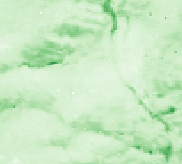
\includegraphics[width=0.2\textwidth]{img_sat/NDVI_1985.png} & 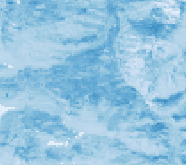
\includegraphics[width=0.2\textwidth]{img_sat/NSI_1985.png} &
    \textbf{1986} & 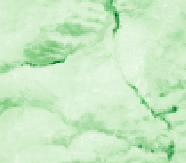
\includegraphics[width=0.2\textwidth]{img_sat/NDVI_1986.png} & 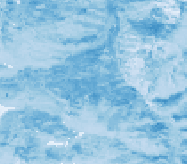
\includegraphics[width=0.2\textwidth]{img_sat/NSI_1986.png} \\
    \hline
    

    \textbf{1987} & \textbf{NO DATA} & \textbf{NO DATA}  &
    \textbf{1988} & 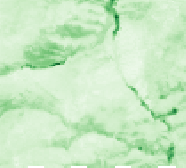
\includegraphics[width=0.2\textwidth]{img_sat/NDVI_1988.png} & 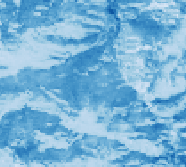
\includegraphics[width=0.2\textwidth]{img_sat/NSI_1988.png} \\
    \hline
    

    \textbf{1989} & 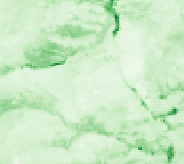
\includegraphics[width=0.2\textwidth]{img_sat/NDVI_1989.png} & 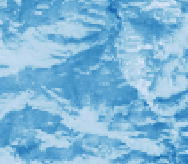
\includegraphics[width=0.2\textwidth]{img_sat/NSI_1989.png} &
    \textbf{1990} & 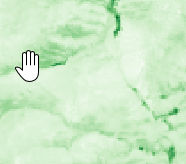
\includegraphics[width=0.2\textwidth]{img_sat/NDVI_1990.png} & 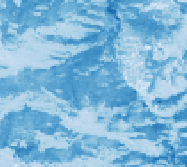
\includegraphics[width=0.2\textwidth]{img_sat/NSI_1990.png} \\
    \hline
    

    \textbf{1991} & 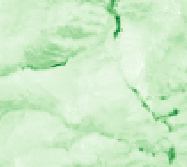
\includegraphics[width=0.2\textwidth]{img_sat/NDVI_1991.png} & 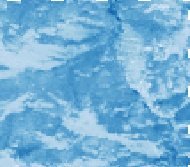
\includegraphics[width=0.2\textwidth]{img_sat/NSI_1991.png} &
    \textbf{1992} & 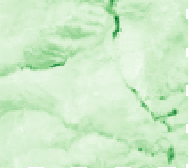
\includegraphics[width=0.2\textwidth]{img_sat/NDVI_1992.png} & 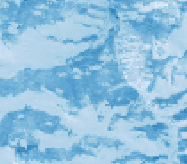
\includegraphics[width=0.2\textwidth]{img_sat/NSI_1992.png} \\
    \hline
    

    \textbf{1993} & 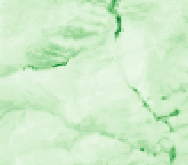
\includegraphics[width=0.2\textwidth]{img_sat/NDVI_1993.png} & 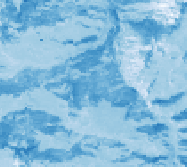
\includegraphics[width=0.2\textwidth]{img_sat/NSI_1993.png} &
    \textbf{1994} & 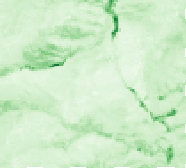
\includegraphics[width=0.2\textwidth]{img_sat/NDVI_1994.png} & 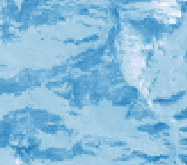
\includegraphics[width=0.2\textwidth]{img_sat/NSI_1994.png} \\
    \hline
    

    \textbf{1995} & 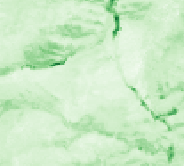
\includegraphics[width=0.2\textwidth]{img_sat/NDVI_1995.png} & 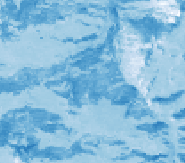
\includegraphics[width=0.2\textwidth]{img_sat/NSI_1995.png} &
    \textbf{1996} & 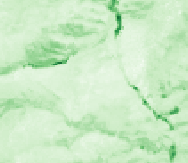
\includegraphics[width=0.2\textwidth]{img_sat/NDVI_1996.png} & 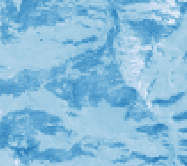
\includegraphics[width=0.2\textwidth]{img_sat/NSI_1996.png} \\
    \hline
    

    \textbf{1997} & 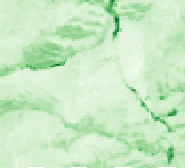
\includegraphics[width=0.2\textwidth]{img_sat/NDVI_1997.png} & 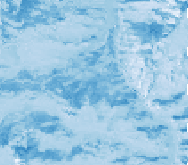
\includegraphics[width=0.2\textwidth]{img_sat/NSI_1997.png} &
    \textbf{1998} & 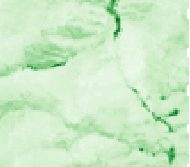
\includegraphics[width=0.2\textwidth]{img_sat/NDVI_1998.png} & 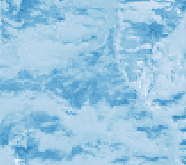
\includegraphics[width=0.2\textwidth]{img_sat/NSI_1998.png} \\
    \hline
    

    \textbf{1999} & 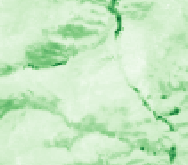
\includegraphics[width=0.2\textwidth]{img_sat/NDVI_1999.png} & 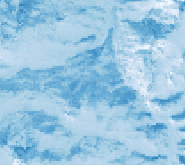
\includegraphics[width=0.2\textwidth]{img_sat/NSI_1999.png} &
    \textbf{2000} & 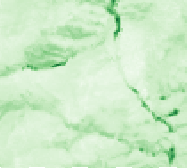
\includegraphics[width=0.2\textwidth]{img_sat/NDVI_2000.png} & 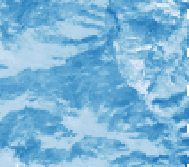
\includegraphics[width=0.2\textwidth]{img_sat/NSI_2000.png} \\
    \hline
    

    \textbf{2001} & 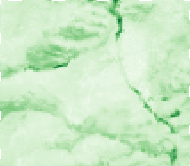
\includegraphics[width=0.2\textwidth]{img_sat/NDVI_2001.png} & 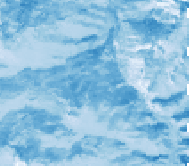
\includegraphics[width=0.2\textwidth]{img_sat/NSI_2001.png} &
    \textbf{2002} & 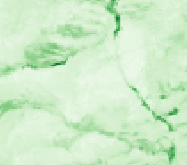
\includegraphics[width=0.2\textwidth]{img_sat/NDVI_2002.png} & 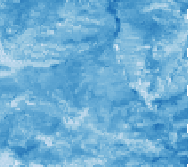
\includegraphics[width=0.2\textwidth]{img_sat/NSI_2002.png} \\
    \hline
    

    \textbf{2003} & 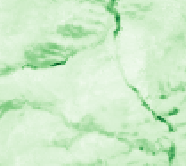
\includegraphics[width=0.2\textwidth]{img_sat/NDVI_2003.png} & 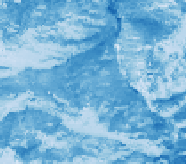
\includegraphics[width=0.2\textwidth]{img_sat/NSI_2003.png} &
    \textbf{2004} & 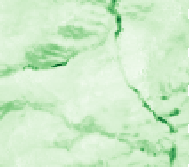
\includegraphics[width=0.2\textwidth]{img_sat/NDVI_2004.png} & 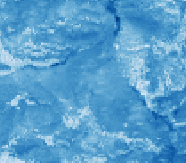
\includegraphics[width=0.2\textwidth]{img_sat/NSI_2004.png} \\
    \hline
    

    \textbf{2005} & 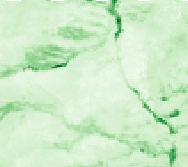
\includegraphics[width=0.2\textwidth]{img_sat/NDVI_2005.png} & 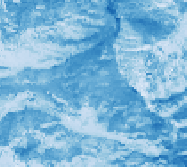
\includegraphics[width=0.2\textwidth]{img_sat/NSI_2005.png} &
    \textbf{2006} & 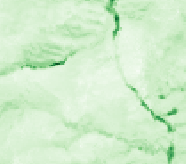
\includegraphics[width=0.2\textwidth]{img_sat/NDVI_2006.png} & 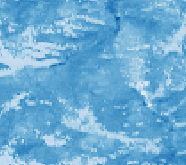
\includegraphics[width=0.2\textwidth]{img_sat/NSI_2006.png} \\
    \hline
    

    \textbf{2007} & 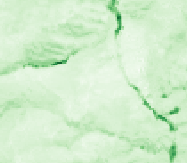
\includegraphics[width=0.2\textwidth]{img_sat/NDVI_2007.png} & 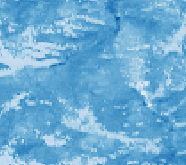
\includegraphics[width=0.2\textwidth]{img_sat/NSI_2007.png} &
    \textbf{2008} & 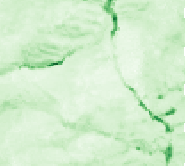
\includegraphics[width=0.2\textwidth]{img_sat/NDVI_2008.png} & 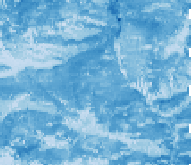
\includegraphics[width=0.2\textwidth]{img_sat/NSI_2008.png} \\
    \hline
    

    \textbf{2009} & 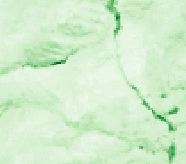
\includegraphics[width=0.2\textwidth]{img_sat/NDVI_2009.png} & 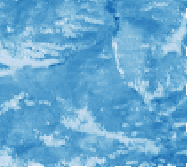
\includegraphics[width=0.2\textwidth]{img_sat/NSI_2009.png} &
    \textbf{2010} & 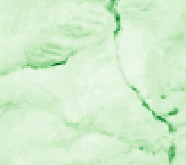
\includegraphics[width=0.2\textwidth]{img_sat/NDVI_2010.png} & 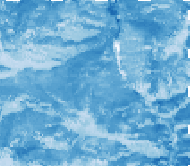
\includegraphics[width=0.2\textwidth]{img_sat/NSI_2010.png} \\
    \hline
    

    \textbf{2011} & \includegraphics[width=0.2\textwidth]{img_sat/NDVI_2011.png} & \includegraphics[width=0.2\textwidth]{img_sat/NSI_2011.png} &
    \textbf{2012} & \textbf{NO DATA} & \textbf{NO DATA} \\
    \hline
    

    \textbf{2013} & \includegraphics[width=0.2\textwidth]{img_sat/NDVI_2013.png} & \includegraphics[width=0.2\textwidth]{img_sat/NSI_2013.png} &
    \textbf{2014} & \includegraphics[width=0.2\textwidth]{img_sat/NDVI_2014.png} & \includegraphics[width=0.2\textwidth]{img_sat/NSI_2014.png} \\
    \hline
    

    \textbf{2015} & \includegraphics[width=0.2\textwidth]{img_sat/NDVI_2015.png} & \includegraphics[width=0.2\textwidth]{img_sat/NSI_2015.png} &
    \textbf{2016} & \includegraphics[width=0.2\textwidth]{img_sat/NDVI_2016.png} & \includegraphics[width=0.2\textwidth]{img_sat/NSI_2016.png} \\
    \hline
    

    \textbf{2017} & \includegraphics[width=0.2\textwidth]{img_sat/NDVI_2017.png} & \includegraphics[width=0.2\textwidth]{img_sat/NSI_2017.png} &
    \textbf{2018} & \includegraphics[width=0.2\textwidth]{img_sat/NDVI_2018.png} & \includegraphics[width=0.2\textwidth]{img_sat/NSI_2018.png} \\
    \hline
    

    \textbf{2019} & \includegraphics[width=0.2\textwidth]{img_sat/NDVI_2019.png} & \includegraphics[width=0.2\textwidth]{img_sat/NSI_2019.png} &
    \textbf{2020} & \includegraphics[width=0.2\textwidth]{img_sat/NDVI_2020.png} & \includegraphics[width=0.2\textwidth]{img_sat/NSI_2020.png} \\
    \hline
    

    \textbf{2019} & \includegraphics[width=0.2\textwidth]{img_sat/NDVI_2019.png} & \includegraphics[width=0.2\textwidth]{img_sat/NSI_2019.png} &
    \textbf{2020} & \includegraphics[width=0.2\textwidth]{img_sat/NDVI_2020.png} & \includegraphics[width=0.2\textwidth]{img_sat/NSI_2020.png} \\
    \hline
    
    % Repite la línea de arriba para cada fila de la tabla
    \end{longtable}

\newpage





\subsection{\textbf{Resultados Estadísticas por Año.}}
En la sección "Tablas de estadísticas para cada imagen por año", se presenta una serie de estadísticas derivadas de las mediciones del Índice de Vegetación de Diferencia Normalizada (NDVI) y del Índice de Nieve Normalizado (NSI) a lo largo de los años.\\

Cada fila de la tabla representa un año distinto, que va desde 1985 hasta 2021. Para cada año, se calculan varias estadísticas para ambos índices, incluyendo la media, la desviación estándar, el valor mínimo y el valor máximo.\\

Las estadísticas del NDVI dan una visión general de la densidad de la vegetación en la región de interés durante cada año. A lo largo del tiempo, se puede observar una variación en los valores medios del NDVI, oscilando desde 0,0686 en 2011 hasta 0,1063 en 2017. La desviación estándar también presenta variaciones, indicando que la densidad de vegetación no es uniforme a lo largo del área y del tiempo.\\ 

Las estadísticas del NSI, por otro lado, proporcionan una idea de la presencia de nieve en la región a lo largo de los años. Los valores medios del NSI varían de 0,0239 en 1999 hasta 0,1644 en 2019, y la desviación estándar muestra una variación similar, reflejando la variabilidad en la cubierta de nieve.\\

Por último, el rango de valores, representado por el mínimo y máximo para cada índice y año, nos da una idea de la dispersión de las mediciones en cada periodo. En el caso del NDVI, los valores máximos muestran una tendencia general al alza desde 0,5366 en 1985 hasta 0,6686 en 2018, mientras que para el NSI los valores máximos varían de 0,1848 en 1985 hasta 0,4082 en 2020.\\

En conjunto, estas estadísticas ofrecen una visión detallada y cuantitativa de las tendencias a largo plazo en la densidad de la vegetación y la cubierta de nieve en la región de interés.\\
{\small

\begin{table}[!ht]
    \centering
    
    \caption{Estadísticas de las imagenes}
    \tiny
    \begin{tabularx}{\textwidth}{XXXXXXXXX}
    \toprule
    \textbf{Año} &  \textbf{mean} \newline \textbf{NDVI} &  \textbf{stddev} \newline \textbf{NDVI} &  \textbf{min} \newline \textbf{NDVI} &  \textbf{max} \newline \textbf{NDVI} &  \textbf{mean} \newline \textbf{NSI} &  \textbf{stddev} \newline \textbf{NSI} &  \textbf{min} \newline \textbf{NSI} &  \textbf{max} \newline \textbf{NSI} \\
    \midrule
    1985 &   0.096263 &     0.057588 & -0.027277 &  0.536563 &  0.031462 &    0.047977 & -0.174510 & 0.184793 \\
    1986 &   0.099113 &     0.062193 & -0.027277 &  0.542233 &  0.031462 &    0.047977 & -0.174510 & 0.184793 \\
    1988 &   0.088367 &     0.058485 & -0.027590 &  0.542029 &  0.108024 &    0.051442 & -0.103631 & 0.278255 \\
    1989 &   0.083763 &     0.055783 & -0.048387 &  0.542029 &  0.079008 &    0.073153 & -0.111615 & 0.311475 \\
    1990 &   0.083863 &     0.054442 & -0.048387 &  0.551853 &  0.070757 &    0.068725 & -0.111615 & 0.305343 \\
    1991 &   0.082345 &     0.052842 & -0.034673 &  0.551853 &  0.065865 &    0.069211 & -0.129046 & 0.305343 \\
    1992 &   0.079993 &     0.051247 & -0.026103 &  0.514689 &  0.085383 &    0.063263 & -0.129046 & 0.305343 \\
    1993 &   0.078426 &     0.050234 & -0.026103 &  0.508556 &  0.037900 &    0.059793 & -0.156916 & 0.281859 \\
    1994 &   0.081826 &     0.052099 & -0.030928 &  0.508556 &  0.055836 &    0.058714 & -0.201351 & 0.230404 \\
    1995 &   0.088023 &     0.054850 & -0.036304 &  0.502358 &  0.054626 &    0.058487 & -0.219512 & 0.230222 \\
    1996 &   0.092122 &     0.055706 & -0.036304 &  0.502358 &  0.056858 &    0.055252 & -0.149327 & 0.230222 \\
    1997 &   0.095284 &     0.061570 & -0.031682 &  0.522075 &  0.024726 &    0.051657 & -0.196685 & 0.199150 \\
    1998 &   0.087817 &     0.058860 & -0.018225 &  0.522075 &  0.027903 &    0.050898 & -0.180464 & 0.206907 \\
    1999 &   0.095901 &     0.069512 & -0.033716 &  0.533603 &  0.023936 &    0.057906 & -0.211004 & 0.214585 \\
    2000 &   0.084066 &     0.057569 & -0.025725 &  0.509402 &  0.074641 &    0.066704 & -0.192067 & 0.254864 \\
    2001 &   0.089655 &     0.060779 & -0.020355 &  0.517510 &  0.042767 &    0.058754 & -0.232652 & 0.225000 \\
    2003 &   0.080137 &     0.060655 & -0.022652 &  0.553300 &  0.098413 &    0.051099 & -0.134860 & 0.316974 \\
    2004 &   0.079954 &     0.062625 & -0.059322 &  0.555007 &  0.077692 &    0.069163 & -0.172227 & 0.301299 \\
    2005 &   0.080983 &     0.061424 & -0.030530 &  0.555007 &  0.136145 &    0.062779 & -0.172227 & 0.370106 \\
    2006 &   0.072828 &     0.054146 & -0.046863 &  0.555007 &  0.070451 &    0.072892 & -0.142325 & 0.301299 \\
    2007 &   0.071206 &     0.053521 & -0.046863 &  0.517546 &  0.100146 &    0.063552 & -0.117615 & 0.320847 \\
    2008 &   0.070293 &     0.053127 & -0.042303 &  0.530632 &  0.084033 &    0.060944 & -0.214867 & 0.320847 \\
    2009 &   0.072027 &     0.053116 & -0.024315 &  0.537978 &  0.108818 &    0.060639 & -0.103504 & 0.320847 \\
    2010 &   0.069392 &     0.050169 & -0.026953 &  0.537978 &  0.096089 &    0.063455 & -0.222120 & 0.285869 \\
    2011 &   0.068617 &     0.049260 & -0.029806 &  0.499324 &  0.097689 &    0.063077 & -0.222859 & 0.269955 \\
    2013 &   0.087995 &     0.064653 & -0.063735 &  0.638094 &  0.120609 &    0.060311 & -0.184541 & 0.371420 \\
    2014 &   0.091166 &     0.064824 & -0.055546 &  0.618061 &  0.049963 &    0.087218 & -0.249169 & 0.346636 \\
    2015 &   0.095457 &     0.070242 & -0.048171 &  0.650983 &  0.048308 &    0.087035 & -0.149120 & 0.345846 \\
    2016 &   0.101752 &     0.076100 & -0.048171 &  0.650834 &  0.034190 &    0.088726 & -0.149120 & 0.342955 \\
    2017 &   0.106304 &     0.082600 & -0.052771 &  0.668613 &  0.059726 &    0.101359 & -0.133595 & 0.345846 \\
    2018 &   0.105001 &     0.081864 & -0.052771 &  0.668613 &  0.141320 &    0.095650 & -0.171782 & 0.377778 \\
    2019 &   0.096551 &     0.071553 & -0.049908 &  0.626652 &  0.164428 &    0.087119 & -0.199741 & 0.408190 \\
    2020 &   0.091125 &     0.063066 & -0.049908 &  0.604941 &  0.161718 &    0.087406 & -0.199741 & 0.408190 \\
    2021 &   0.089626 &     0.061294 & -0.050851 &  0.583714 &  0.143477 &    0.089564 & -0.201038 & 0.372990 \\
    \bottomrule
    \end{tabularx}
\end{table}

}
\clearpage

\subsection{\textbf{Graficas comparativas NDVI y NSI.}}
Los datos presentados aquí  graficados representan valores promedio anuales, mínimos, máximos y desviación estándar de los índices de vegetación NDVI y NSI desde 1985 hasta 2021. En general, vemos fluctuaciones en estos valores a lo largo del tiempo, con algunas tendencias y anomalías notables.\\

Examinando los datos, vemos que no siempre hay una correlación directa entre los valores promedio de NDVI y NSI en un año determinado. Por ejemplo, en 1988, el valor promedio de NDVI disminuyó en comparación con 1986, mientras que el valor promedio de NSI aumentó significativamente. Este tipo de discrepancias podrían ser el resultado de diferentes respuestas de los dos índices a las condiciones ambientales específicas de ese año.\\

Además, hay algunos años que destacan por tener valores que difieren significativamente de los años circundantes. Por ejemplo, en 2018, el valor promedio de NSI es notablemente más alto que en los años anteriores y posteriores. Si bien estos datos no nos dicen la causa exacta de estas anomalías, sugieren que hubo cambios en la vegetación o en las condiciones ambientales durante estos años que merecen una investigación más detallada.\\

En cuanto a la variabilidad anual de los valores de NDVI y NSI, medida por la desviación estándar, vemos que hay variaciones significativas de un año a otro. Un mayor valor de desviación estándar indica que hubo una mayor variabilidad en los valores de NDVI o NSI dentro de ese año. Por ejemplo, en 2017, el valor de desviación estándar del NDVI es particularmente alto, lo que sugiere una amplia gama de valores de NDVI en las imágenes capturadas, como ventana, ese año. Esta variabilidad puede estar relacionada con factores como variaciones estacionales o cambios en las condiciones ambientales.\\

En resumen, estos datos proporcionan una visión útil de cómo los valores de NDVI y NSI han fluctuado a lo largo del tiempo. Sin embargo, es importante tener en cuenta que estos índices son solo una representación de la vegetación y pueden ser influenciados por una variedad de factores. Además, los patrones y tendencias observados en estos datos nos permiten formular hipótesis para futuras investigaciones\\


\begin{figure}[H]
    \centering
    \includegraphics[width=1.1\textwidth]{img_stats/graficas.png}
    \caption{Comparativos estadísticas NDVI y NSI}
    \label{fig:comparativos estadísticas NDVI y NSI}
\end{figure}


\newpage

\subsection{\textbf{Correlaciones entre las variables}}
Hemos realizado un análisis de correlación para investigar la relación entre las diferentes variables de nuestro conjunto de datos. Los resultados se presentan en la matriz de correlación.\\

La correlación entre dos variables puede variar entre -1 y 1. Un valor de correlación cercano a 1 indica una fuerte correlación positiva, lo que significa que si una variable aumenta, la otra también tiende a aumentar. Por otro lado, un valor cercano a -1 indica una fuerte correlación negativa, lo que significa que si una variable aumenta, la otra tiende a disminuir. Un valor cercano a 0 indica una correlación débil o inexistente entre las variables.\\

Los valores de NDVI y NSI muestran algunas correlaciones interesantes con respecto al tiempo y entre sí. Algunas de las observaciones clave de esta matriz de correlación son:\\
\begin{enumerate}
\item\textbf{Desviación estándar de NDVI y valor máximo de NDVI (0.839):} Se observa una fuerte correlación positiva, sugiriendo que en años con mayor variabilidad en la vegetación, es más probable que veamos valores de NDVI más altos. Esto podría indicar que las condiciones que llevan a una mayor diversidad de vegetación también permiten la existencia de áreas con una vegetación excepcionalmente vigorosa.\\

\item\textbf{Desviación estándar de NDVI y año (0.525728):}
La correlación positiva aquí sugiere que la variabilidad en la vegetación ha aumentado con el tiempo. Esto podría ser un reflejo de cambios más amplios en las condiciones climáticas o de la tierra.\\

\item\textbf{Valor máximo de NSI y año (0.741803):}
Esta fuerte correlación positiva indica que los niveles máximos de nieve han ido en aumento a lo largo de los años. Esto podría reflejar tendencias más amplias en las condiciones climáticas, como aumentos en las precipitaciones invernales.\\

\item\textbf{Valor máximo de NSI y valor medio de NSI (0.763314):} 
Esta fuerte correlación positiva implica que los años con un valor medio más alto de nieve también tienden a tener un valor máximo más alto. Esto puede sugerir que los factores que influyen en el nivel medio de nieve también afectan la probabilidad de experimentar niveles de nieve extremadamente altos\\

\item\textbf{Desviación estándar de NSI y año (0.736978): } 
Esta correlación fuerte y positiva indica que la variabilidad en los niveles de nieve ha aumentado a lo largo del tiempo. Esto puede reflejar la influencia de los cambios climáticos, que pueden estar aumentando la variabilidad en las precipitaciones de nieve.\\

\item\textbf{Valor máximo de NSI y desviación estándar de NSI (0.749685):} 
Esta correlación fuerte y positiva sugiere que en los años con una mayor variabilidad en los niveles de nieve, también es más probable que se vea un valor máximo más alto de NSI. Esto podría indicar que las condiciones climáticas más variables también aumentan la probabilidad de experimentar niveles de nieve extremadamente altos\\
\item\textbf{Máximo de NDVI y la desviación estándar de NSI (0.797) :} 
Esta fuerte correlación positiva indica que en los años con una mayor variabilidad en los niveles de nieve (medida por la desviación estándar de NSI), también se tiende a ver un valor máximo más alto de NDVI, que es una medida de la vegetación.\\  

\end{enumerate}

En general, estos resultados muestran que existen algunas relaciones interesantes entre las variables de NDVI y NSI y cómo han cambiado a lo largo del tiempo. Sin embargo, se necesitaría más investigación para entender completamente las causas detrás de estas correlaciones.\\


\begin{figure}[H]
    \centering
    \includegraphics[width=0.8\textwidth]{img_stats/matriz_correlacion.png}
    \caption{Matriz de correlación}
    \label{fig:matriz de correlacion}
\end{figure}


\newpage
\subsection{\textbf{Resultados del Test de Tendencias Temporales}}
{\small

\begin{enumerate}
    \item \textbf{Media NDVI:}
    \begin{align*}
        &\text{Pendiente: } 0.000109 \\
        &\text{Valor p: } 0.514211
    \end{align*}
    La pendiente es positiva, lo que indica una tendencia ascendente en la media del NDVI a lo largo del tiempo. Sin embargo, el valor p es mayor a 0.05, lo que sugiere que esta tendencia no es estadísticamente significativa.

    \item \textbf{Desviación estándar NDVI:}
    \begin{align*}
        &\text{Pendiente: } 0.000415 \\
        &\text{Valor p: } 0.001407
    \end{align*}
    La pendiente es positiva, lo que indica que la variabilidad del NDVI está aumentando a lo largo del tiempo. El valor p es menor a 0.05, lo que sugiere que esta tendencia es estadísticamente significativa.\\

    \item \textbf{Mínimo NDVI:}
    \begin{align*}
        &\text{Pendiente: } -0.000638 \\
        &\text{Valor p: } 0.000697
    \end{align*}
    La pendiente es negativa, lo que indica una tendencia descendente en el valor mínimo del NDVI a lo largo del tiempo. El valor p es menor a 0.05, lo que sugiere que esta tendencia es estadísticamente significativa.\\
    
    \item \textbf{Máximo NDVI:}
    \begin{align*}
        &\text{Pendiente: } 0.003235 \\
        &\text{Valor p: } 9.133e-06
    \end{align*}
    La pendiente es positiva, lo que indica una tendencia ascendente en el valor máximo del NDVI a lo largo del tiempo. El valor p es muy pequeño, lo que sugiere que esta tendencia es altamente estadísticamente significativa.\\

    \item \textbf{Media NSI:}
    \begin{align*}
        &\text{Pendiente: } 0.001978 \\
        &\text{Valor p: } 0.001058
    \end{align*}
    La pendiente es positiva, lo que indica una tendencia ascendente en la media del NSI a lo largo del tiempo. El valor p es menor a 0.05, lo que sugiere que esta tendencia es estadísticamente significativa.\\

    \item \textbf{Desviación estándar NSI:}
    \begin{align*}
        &\text{Pendiente: } 0.000995 \\
        &\text{Valor p: } 6.682335e-07
    \end{align*}
    La pendiente es positiva, lo que indica que la variabilidad del NSI está aumentando a lo largo del tiempo. El valor p es muy pequeño, lo que sugiere que esta tendencia es altamente estadísticamente significativa.\\

    \item \textbf{Mínimo NSI:}
    \begin{align*}
        &\text{Pendiente: } -0.0010974 \\
        &\text{Valor p: } 0.090237
    \end{align*}
    La pendiente es negativa, lo que indica una tendencia descendente en el valor mínimo del NSI a lo largo del tiempo. Sin embargo, el valor p es mayor a 0.05, lo que sugiere que esta tendencia no es estadísticamente significativa.\\

    \item \textbf{Máximo NSI:}
    \begin{align*}
        &\text{Pendiente: } 0.004314 \\
        &\text{Valor p: } 5.163803e-07
    \end{align*}
    La pendiente es positiva, lo que indica una tendencia ascendente en el valor máximo del NSI a lo largo del tiempo. El valor p es muy pequeño, lo que sugiere que esta tendencia es altamente estadísticamente significativa.\\
\end{enumerate}
}

